To evaluate the API, the implementation must be first compared to the requirements defined in
Chapter~\ref{ch:analysis/requirements}.
If the API fails to meet these requirements, the API has failed to address the issues with BSD Sockets discussed in
Section~\ref{sec:bsd-sockets}.
Secondly, a direct comparison with BSD Sockets will be conducted to determine if the API has actually resulted in a
better API for modern network programming.

\section{Requirements Matching}\label{sec:requirements-matching}
A key issue discussed with BSD Sockets is the lack of compile time safety due to being an integer-based API written in
the C programming language.
This lead to the required functional requirement for sending and receiving typed messages exclusively, as well as the
optional functional requirement for a compile-time check to ensure the user has specified the correct \Endpoint{}s to
be able to initiate a \connection{} or bind a \listener{}.
Both of these requirements have been successfully implemented.
Typed messages are enforce through the requirement of a \framer{} for a \connection{}, and the \framer{}'s associated
types \texttt{Input} and \texttt{Output}.
The \connection{}'s \texttt{send()} method requires the \connection{}'s \framer{}'s \texttt{Input} type to be given and
the \connection{}'s \texttt{recv()} method can only decode messages which are of the same type as the \connection{}'s
\framer{}'s \texttt{Output} type.
To ensure the correct \Endpoint{}s are specified, the \preconnection{} is implemented as a state machine, which only
allows the user to call specific methods when the correct \Endpoint{}s are given.
See Section~\ref{sec:preconnection-endpoint-safety} for details on the state machine.

Another issue discussed with BSD Sockets is its synchronous nature, which fails to represent the true nature of
networks.
This lead to the required functional requirement for the API to be asynchronous where possible, utilising Rust's
\texttt{Future}s mechanism.
Through the use of Rust's Tokio library as discussed in Section~\ref{sec:tokio}, all I/O operations are forced to make
use of Rust's \asyncawait{} which produces \texttt{Future}s.
These \texttt{Future}s are manipulated within the API and passed to the user.
See Section~\ref{sec:rust} and Section~\ref{sec:connection-racing-impl} for details.

To ensure the API is usable, a required function requirement was specified which required a simple client-server example
must be implemented.
This resulted in a HTTP example in which the client requested a TOML\footnote{Tom's Obvious, Minimal Language -
    \url{https://github.com/toml-lang/toml}} which is evaluated in detail in Section~\ref{subsec:api-comparison}.

Due to the nature of networks, messages cannot be assumed to arrive in one piece, rather may require multiple attempts
to receive the full message.
BSD Sockets requires the user too repeatedly call \texttt{recv()} until the user determined the data is complete.
The TAPS specification allows for an API to produce a partial message, which the user may choose to attempt to request
more data from the remote to complete the message or not.
This lead to an optional functional requirement for the API to be able to handle partial messages.
While the API doesn't allow for partial messages in the same way as the TAPS specification, it can handle incomplete
messages from the underlying transport layer.
This is discussed in detail in Section~\ref{sec:receiving-messages}, but does not fully fufill the requirement.
The user may wish to handle partial messages themselves, which this method does not allow.
Furthermore, if the underlying transport layer is unreliable, such as UDP, the \texttt{Future} from a \texttt{recv()}
call may never complete, since the API assumes the transport layer will request the missing data from the remote.

A common use case of networks is to transfer large amounts of data of an unknown size.
BSD Sockets leaves handling this to the user, which can be error prone.
This lead to an optional functional requirement for the API to be ale to send messages of unknown size.
Support for this is not explicit in the API, and has not been directly implemented, but since the \encode{} and
\decode{} traits do not enforce the messages to have a known size, it can be implemented in theory.
The \decode{} trait does have a requirement the type also implements \texttt{Sized}, which ensures the type has a known
compile time stack size.
This only requires the type have a known stack size, not a known heap size, for example Rust's heap-allocated array
type \texttt{Vec} has a known stack size of 3 words, but has an unknown heap size at compile time.

An API which could only send and receive types which the API had defined leads to a restrictive API with limited
potential uses.
This lead to the required non-functional requirement for the API to allow user-defined types to be used
Through the use of the \encode{} and \decode{} traits, the user can send and receive their own types with a
\connection{} object.
These traits define a type which can be converted to and from the raw bytes the underlying transport layer uses.
See Section~\ref{subsec:encode-and-decode} for details on these traits.

To reduce the learning curve for an API, the API should be “self-documenting'', meaning the names of types and methods
should describe their use and function at a high-level, without having to read explicit documentation.
This lead to the required non-functional requirement for the API to be “self-documenting''.
Many of the types and function names are inherited from the TAPS specification, which are ``self-documenting''.
This coupled with the use of existing design patterns like the builder pattern, programs written with the API are easy
to understand at a glance.
See Section~\ref{subsec:api-comparison} for a detailed comparison between the API and BSD Sockets.

\section{Comparison to BSD Sockets}\label{sec:comparison-to-bsd-sockets}

\subsection{API Comparison}\label{subsec:api-comparison}
\lstinputlisting[float=h, label=lst:client, caption={A HTTP Client example which sends a GET request for a Cargo.toml
file and outputs the name within in.}]{../data/client.rs}
\lstinputlisting[float=h, label=lst:server, caption={A HTTP Server example which listens for a GET request for
Cargo.toml and send the file as a response.}]{../data/server.rs}

\begin{lstlisting}[float=h, caption={The compiler error produced if a Preconnection without a remote endpoint is used to
initiate a Connection.}, label=lst:clientError]
error[E0599]: no method named `initiate` found for struct `taps::preconnection::Preconnection<taps::http::client::HttpClient<_, _>, taps::preconnection::NoEndpoint, taps::preconnection::NoEndpoint>` in the current scope
\end{lstlisting}

\begin{lstlisting}[float=h, caption={The compiler error produced if a Preconnection without a local endpoint is used to
listen for Connections.}, label=lst:serverError]
error[E0599]: no method named `listen` found for struct `taps::preconnection::Preconnection<taps::http::client::HttpServer<_, _>, taps::preconnection::NoEndpoint, taps::preconnection::NoEndpoint>` in the current scope
\end{lstlisting}

In terms of complexity of the user's code, the API resulting more succinct code which follows a user's reasoning of how
a connection works.
Whereas an implementation using BSD Sockets would result in at least an order of magnitude more code, leading to
increased code complexity.
Appendix~\ref{ch:bsd-sockets-connection-code} is \(134\) lines long using BSD Sockets, whereas
Appendix~\ref{ch:taps-connection-evaluation-code} is 21 lines long with TAPS .
At a glance, the TAPS version is easier to understand as the optional requirement of a “self-documenting” API has been
met by ensuring all methods concisely describe what they do, and methods can be chained together fluently to represent
the flow of the program.

\subsection{Latency Comparison}\label{sec:latency-comparison}
Performance is important for network programming, and as discussed in Chapter~\ref{ch:analysis/requirements} the new
API should have performance similar to BSD Sockets (Sockets).
A major difference between the two API is how they open connections.
This API does similar things to the Sockets version, but does them internally and asynchronously.
For example, the Sockets version requires the user to explicitly resolve domain names and race them, whereas TAPS
does this internally.
Since this difference could be significant, a test will be ran to determine which API has the lowest time for opening
connections.
For this comparison, two implementations of a program which attempts a DNS lookup for a given domain name and connects
to first successful connection attempt, prioritising IPv6 addresses over IPv4 addresses.
To have a fair comparison between the two APIs, the BSD Sockets version must also prioritise IPv6 addresses over IPv4
addresses, since the TAPS version does this internally.
Since a DNS lookup could have a large impact on the total latency, the domain tested is requested multiple times before
running the program under test.
The tests will be executed on a University-provided Linux machine, connected to the University's IPv6 enabled network.
See Appendix~\ref{ch:bash-script-for-latency-testing} for the script used to test the two programs.

\begin{figure}[h]
    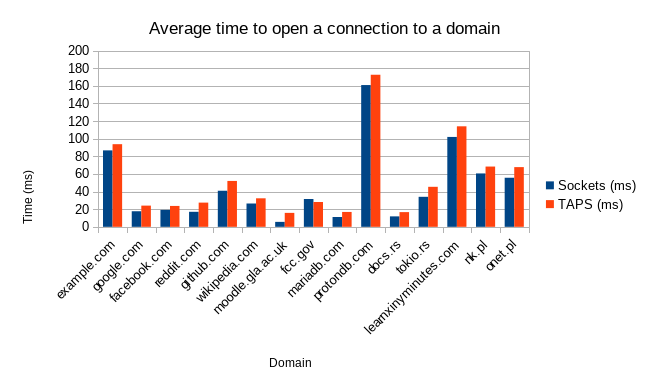
\includegraphics[width=\textwidth]{../data/processed/avg_latency}
    \caption{A graph to show the average time each API takes to connect to a range of domains.}
    \label{fig:latency}
\end{figure}

As shown in Figure~\ref{fig:latency}, TAPS is slightly slower at opening connections in almost every case when compared
to Sockets.
This is likely due to TAPS being an asynchronous API.
For the \texttt{Future}'s to be executed, an asynchronous runtime must be created to repeatedly poll each
\texttt{Future}.
Sockets does not have this overhead since it is a synchronous API.
To reduce the impact of this overhead, the programs were modified to open \(10\) connections each time they were run.

\begin{figure}[h]
    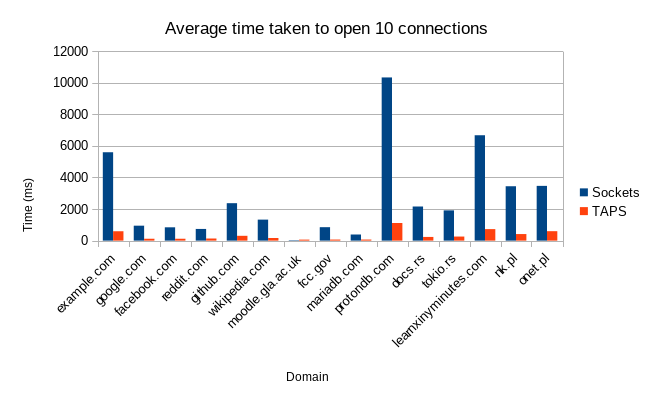
\includegraphics[width=\textwidth]{../data/processed/avg_multi}
    \caption{A graph to show the average time each API takes to open 10 connections to a range of domains.}
    \label{fig:multiLatency}
\end{figure}

Figure~\ref{fig:multiLatency} shows the results of the test after the programs were modified and shows TAPS is takes
less time to open \(10\) connections.
This will be because each connection attempt is executed asynchronously, whereas the Sockets version opens each
connection sequentially.

As a result of the two tests, Sockets has been shown to have a lower connection-initialisation latency, therefore would
be better suited for short-lived programs, which open a few connections, or programs which would not benefit from an
asynchronous runtime, such as simple single-threaded programs.
An example of this type of program would be cURL\footnote{\url{https://curl.haxx.se}} or
wget\footnote{\url{https://www.gnu.org/software/wget/}}.
Whereas, TAPS would be better suited for programs which open many connections, and can make use of the asynchronous
runtime.
An example would be Firefox\footnote{\url{https://www.mozilla.org/en-US/firefox/}} or qBittorrent
\footnote{\url{https://www.qbittorrent.org}}.

%\subsection{Code Comparison}\label{subsec:lines-of-code-comparison}
%While lines of code is not a good metric to determine the quality of code, the substantial difference between the two
%implementations is worth discussing.
%Since sockets is a lower level library than TAPS, more code is required to do the same work as in TAPS .
%Opening a connection with the sockets API requires the following:
%\begin{itemize}
%    \item DNS lookup via \texttt{getaddrinfo}
%    \item Reorder DNS responses to prioritise IPv6 addresses
%    \item Open a socket
%    \item Connect to the remote server
%\end{itemize}
%The TAPS API does this all within \emph{Preconnection}'s \texttt{initiate} method.

%How good is your solution? How well did you solve the general problem, and what evidence do you have to support that?
%
%\section{Guidance}
%\begin{itemize}
%    \item
%        Ask specific questions that address the general problem.
%    \item
%        Answer them with precise evidence (graphs, numbers, statistical
%        analysis, qualitative analysis).
%    \item
%        Be fair and be scientific.
%    \item
%        The key thing is to show that you know how to evaluate your work, not
%        that your work is the most amazing product ever.
%\end{itemize}
%
%\section{Evidence}
%Make sure you present your evidence well. Use appropriate visualisations, reporting techniques and statistical analysis, as appropriate.
%
%If you visualise, follow the basic rules, as illustrated in Figure~\ref{fig:boxplot}:
%\begin{itemize}
%\item Label everything correctly (axis, title, units).
%\item Caption thoroughly.
%\item Reference in text.
%\item \textbf{Include appropriate display of uncertainty (e.g. error bars, Box plot)}
%\item Minimize clutter.
%\end{itemize}
%
%See the file \texttt{guide\_to\_visualising.pdf} for further information and guidance.
%
%\begin{figure}
%    \centering
%    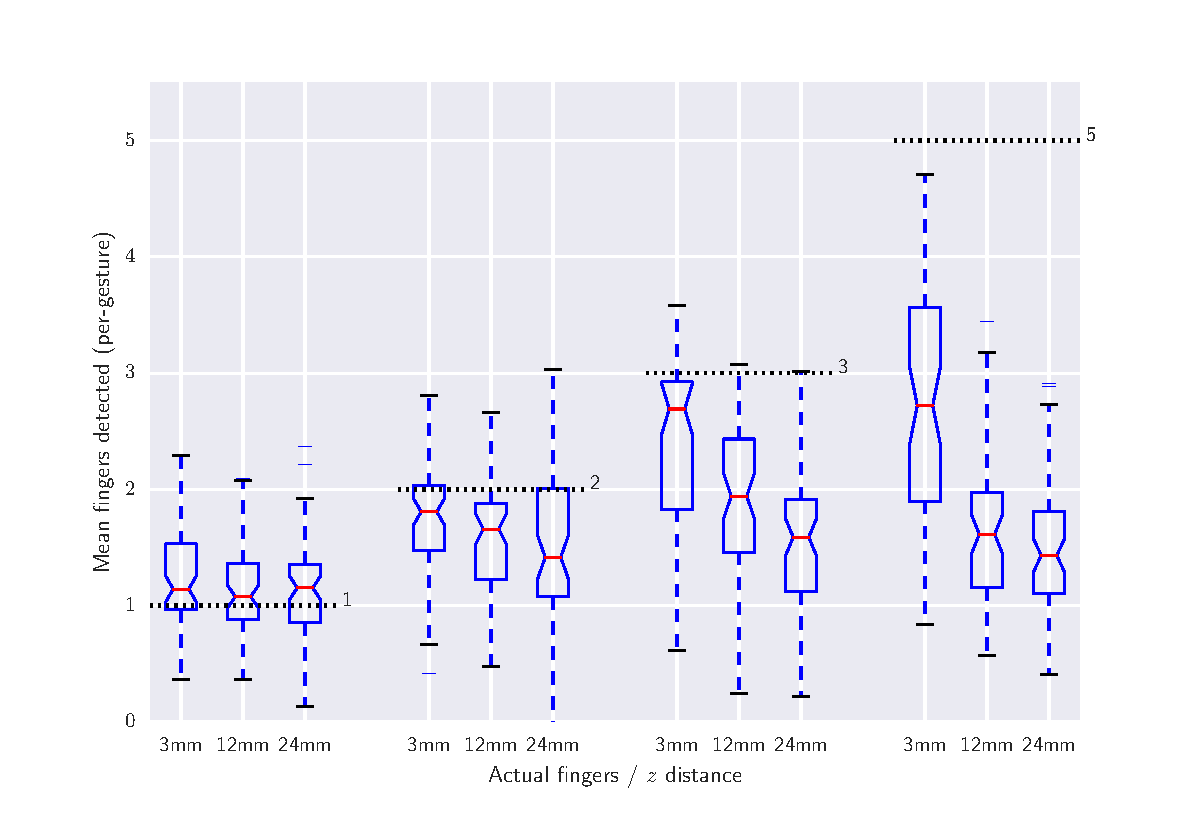
\includegraphics[width=1.0\linewidth]{images/boxplot_finger_distance.pdf}
%
%    \caption{Average number of fingers detected by the touch sensor at different heights above the surface, averaged over all gestures. Dashed lines indicate
%    the true number of fingers present. The Box plots include bootstrapped uncertainty notches for the median. It is clear that the device is biased toward
%    undercounting fingers, particularly at higher $z$ distances.
%    }
%
%    % use the notation fig:name to cross reference a figure
%    \label{fig:boxplot}
%\end{figure}
